\newif\ifshowsolutions
\showsolutionstrue
\documentclass{article}
\usepackage{listings}
\usepackage{amsmath}
\usepackage{subfig}
\usepackage{amsthm}
\usepackage{amsmath}
\usepackage{amssymb}
\usepackage{graphicx}
\usepackage{mdwlist}
\usepackage{geometry}
\usepackage{titlesec}
\usepackage{palatino}
\usepackage{mathrsfs}
\usepackage{fancyhdr}
\usepackage{paralist}
\usepackage{todonotes}
\usepackage{tikz}
\usepackage{float} % Place figures where you ACTUALLY want it
\usepackage{comment} % A hack to toggle sections
\usepackage{ifthen}
\usepackage{mdframed}
\usepackage{verbatim}
\usepackage{listings}
\usepackage{bbm}
\usepackage{upquote} % Prevents backticks replacing single-quotes in verbatim
\usepackage[strings]{underscore}
\usepackage[colorlinks=true]{hyperref}
\usetikzlibrary{positioning,shapes,backgrounds}

\geometry{margin=1in}
\geometry{headheight=2in}
\geometry{top=2in}

\setlength{\marginparwidth}{2.15cm}
\setlength{\parindent}{0em}
\setlength{\parskip}{0.6\baselineskip}

\rhead{}
\lhead{}

% Spacing settings.
\titlespacing\section{0pt}{12pt plus 2pt minus 2pt}{0pt plus 2pt minus 2pt}
\titlespacing\subsection{0pt}{12pt plus 4pt minus 2pt}{0pt plus 2pt minus 2pt}
\titlespacing\subsubsection{0pt}{12pt plus 4pt minus 2pt}{0pt plus 2pt minus 2pt}
\renewcommand{\baselinestretch}{1.15}

% Shortcuts for commonly used operators.
\newcommand{\E}{\mathbb{E}}
\newcommand{\Var}{\operatorname{Var}}
\newcommand{\Cov}{\operatorname{Cov}}
\newcommand{\Bias}{\operatorname{Bias}}
\DeclareMathOperator{\argmin}{arg\,min}
\DeclareMathOperator{\argmax}{arg\,max}

% Do not number subsections and below.
\setcounter{secnumdepth}{1}

% Custom format subsection.
\titleformat*{\subsection}{\large\bfseries}

% Set up the problem environment.
\newcounter{problem}[section]
\newenvironment{problem}[1][]
  {\begingroup
    \setlength{\parskip}{0em}
    \refstepcounter{problem}\par\addvspace{1em}\textbf{Problem~\Alph{problem}\!
    \ifthenelse{\equal{#1}{}}{}{ [#1 points]}:}
  \endgroup}

% Set up the subproblem environment.
\newcounter{subproblem}[problem]
\newenvironment{subproblem}[1][]
  {\begingroup
    \setlength{\parskip}{0em}
    \refstepcounter{subproblem}\par\medskip\textbf{\roman{subproblem}.\!
    \ifthenelse{\equal{#1}{}}{}{ [#1 points]:}}
  \endgroup}

% Set up the teachers and materials commands.
\newcommand\teachers[1]
  {\begingroup
    \setlength{\parskip}{0em}
    \vspace{0.3em} \textit{\hspace*{2em} TAs responsible: #1} \par
  \endgroup}
\newcommand\materials[1]
  {\begingroup
    \setlength{\parskip}{0em}
    \textit{\hspace*{2em} Relevant materials: #1} \par \vspace{1em}
  \endgroup}

% Set up the hint environment.
\newenvironment{hint}[1][]
  {\begin{em}\textbf{Hint: }}
  {\end{em}}

% Set up the solution environment.
\ifshowsolutions
  \newenvironment{solution}[1][]
    {\par\medskip \begin{mdframed}\textbf{Solution~\Alph{problem}#1:} \begin{em}}
    {\end{em}\medskip\end{mdframed}\medskip}
  \newenvironment{subsolution}[1][]
    {\par\medskip \begin{mdframed}\textbf{Solution~\Alph{problem}#1.\roman{subproblem}:} \begin{em}}
    {\end{em}\medskip\end{mdframed}\medskip}
\else
  \excludecomment{solution}
  \excludecomment{subsolution}
\fi



%%%%%%%%%%%%%%%%%%%%%%%%%%%%%%
% HEADER
%%%%%%%%%%%%%%%%%%%%%%%%%%%%%%

\chead{
  {\vbox{
      \vspace{2mm}
      \large
      Caltech CS/CNS/EE 155 \hfill
      Philip Carr \hfill \\[1pt]
      Set 5\hfill
      February 2019\\
    }
  }
}

\begin{document}
\pagestyle{fancy}



\section{SVD and PCA [35 Points]}

\problem[3] 

\begin{solution}\normalfont{
The principal components of $X$ are the vectors $u_1, u_2, \dots, u_n$ such that $XX^T = U\Lambda U^T$, where $U = [u_1\,u_2\,\cdots\,u_n]$ and $\Lambda$ is a diagonal matrix with the eigenvalues of $XX^T$ along the diagonal. Given the singular value decomposition (SVD) decomposition $X = U\Sigma V^T$, $XX^T = (U\Sigma V^T)(U\Sigma V^T)^T = U\Sigma V^T V \Sigma^T U^T$. Since $V$ is orthogonal, $U\Sigma V^T V \Sigma^T U^T = U\Sigma \Sigma^T U^T = U\Sigma^2 U^T = U\Lambda U^T$. Thus, the columns of $U$ are the principal components of $X$, where $\Lambda = \Sigma^2$, and thus the singular values of $X$ are the square roots of the eigenvalues of $XX^T$.
}\end{solution}

\newpage
\problem[4] 

\begin{solution}\normalfont{
Intuitive explanation: Since the feature covariance matrix $\Sigma$ is expressed as $\Sigma = XX^T = U\Lambda U^T$, the diagonal terms of $\Sigma$, $\Sigma_{dd}$, correspond to the covariances of feature $d$ with itself in the training data, which are non-negative for all features $d$. Therefore, all the diagonal terms of $\Lambda$, which are the eigenvalues of the PCA of $X$, are non-negative.\\
\\
Mathematical explanation: Since the eigenvalues of the PCA of $X$ are the squares of the singular values of the SVD of $X$, the eigenvalues of the PCA of $X$ must be non-negative.
}\end{solution}

\newpage
\problem[5] 

\begin{solution}\normalfont{
Using the definition of matrix multiplication, $C = AB$ where $c_{ij} = \sum_{k=1}^m a_{ik}b_{kj}$ where $m$ is the number of columns of $A$ and the number of rows of $B$, $\text{Tr}(AB) = \sum_{i=1}^N(AB)_{ii} = \sum_{i=1}^N(\sum_{j=1}^N a_{ij}b_{ji}) = \sum_{i=1}^N(\sum_{j=1}^N b_{ji}a_{ij}) = \sum_{j=1}^N(\sum_{i=1}^N b_{ji}a_{ij}) = \sum_{i=1}^N(BA)_{ii} = \text{Tr}(BA)$.\\
\\
Generalizing to square matrices $A$, $B$, and $C$,
\[ \text{Tr}(ABC) = \sum_{i=1}^N(ABC)_{ii} = \sum_{i=1}^N\sum_{k=1}^N(AB)_{ik}C_{ki} = \sum_{i=1}^N(\sum_{k=1}^N(\sum_{j=1}^N a_{ij}b_{jk})c_{ki}) = \sum_{i=1}^N \sum_{k=1}^N \sum_{j=1}^N a_{ij}b_{jk} c_{ki} \]
\[ = \sum_{i=1}^N \sum_{k=1}^N \sum_{j=1}^N a_{ij}(b_{jk} c_{ki}) = \sum_{i=1}^N \sum_{k=1}^N \sum_{j=1}^N (b_{jk} c_{ki})a_{ij} = \sum_{j=1}^N (\sum_{i=1}^N (\sum_{k=1}^N b_{jk} c_{ki})a_{ij}) = \sum_{j=1}^N\sum_{i=1}^N(BC)_{ji}A_{ij} \]
\[ = \sum_{j=1}^N(BCA)_{jj} = \text{Tr}(BCA). \]
\\
Furthermore,
\[ \text{Tr}(BCA) = \sum_{i=1}^N(BCA)_{ii} = \sum_{i=1}^N\sum_{k=1}^N(BC)_{ik}A_{ki} = \sum_{i=1}^N(\sum_{k=1}^N(\sum_{j=1}^N b_{ij}c_{jk})a_{ki}) = \sum_{i=1}^N \sum_{k=1}^N \sum_{j=1}^N b_{ij}c_{jk} a_{ki} \]
\[ = \sum_{i=1}^N \sum_{k=1}^N \sum_{j=1}^N b_{ij}(c_{jk} a_{ki}) = \sum_{i=1}^N \sum_{k=1}^N \sum_{j=1}^N (c_{jk} a_{ki})b_{ij} = \sum_{j=1}^N (\sum_{i=1}^N (\sum_{k=1}^N c_{jk} a_{ki})b_{ij}) = \sum_{j=1}^N\sum_{i=1}^N(CA)_{ji}B_{ij} \]
\[ = \sum_{j=1}^N(CAB)_{jj} = \text{Tr}(CAB). \]
Therefore, $\text{Tr}(ABC) = \text{Tr}(BCA) = \text{Tr}(CAB)$ holds for any square matrices $A$, $B$, and $C$.
}\end{solution}

\newpage
\problem[3] 

\begin{solution}\normalfont{
To store a truncated SVD with $k$ singular values, the first $k$ columns of $U$, the first $k$ singular values in $\Sigma$ are needed, and the first $k$ rows of $V^T$ are needed. Therefore, To store a truncated SVD with $k$ singular values of an $N \times N$ matrix $X$, $Nk + k + Nk = (2N + 1)k$ values are needed.
}\end{solution}


\newpage
\problem[3] .

\begin{solution}\normalfont{
Since $X$ has rank $N < D$, the values along the diagonal in $\Sigma$ are 0. Therefore, the only nonzero entries of $\Sigma$ are $\Sigma_{ii}$ where $i \leq N$. Using the definition of matrix multiplication (see problem 1C),
\[ (U\Sigma)_{ij} = \sum_{k=1}^D U_{ik}\Sigma_{kj} = \sum_{k=1}^N U_{ik}\Sigma_{kj} + \sum_{k=N+1}^D U_{ik}\Sigma_{kj} = \sum_{k=1}^N U_{ik}\Sigma_{kj} + \sum_{k=N+1}^D U_{ik}(0) = \sum_{k=1}^N U_{ik}\Sigma_{kj} = (U'\Sigma')_{ij}, \]
where $U'$ is the $D \times N$ matrix consisting of the first $N$ columns of $U$, and where $\Sigma'$ is the $N \times N$ matrix consisting of the first $N$ rows of $\Sigma$. Therefore, $U\Sigma = U'\Sigma'$.
}\end{solution}

\newpage
\problem[3] 

\begin{solution}\normalfont{
Since $U'$ is not square, $U'U'^T$ has different dimensions from $U'^TU'$, so $U'U'^T \neq U'^TU'$. Since a matrix $A$ is orthogonal if $AA^T = A^TA = I$, because $U'$ is not square, $U'$ is not orthogonal.
}\end{solution} 

\newpage
\problem[4] 

\begin{solution}\normalfont{
The $ij$-th entry of $U'^TU'$ is the dot product of vectors $u_i$ and $u_j$, where $u_i^T$ is the $i$th row of $U'^T$, and $u_j$ is the $j$th column of $U'$. If $i = j$, since $U'$ has orthonormal columns, then $u_i \cdot u_j = u_i \cdot u_i = 1$, so every $ii$-th entry of $U'^TU'$ is 1. If $i \neq j$, $u_i \cdot u_j = 0$, so so every $ij$-th entry of $U'^TU'$ where $i \neq j$ is 0. Since $U'^TU'$ has dimensions $N \times N$, $U'^TU' = I_{N\times N}$.\\
\\
Assume $U'U'^T = I_{D \times D}$. Thus, the $ij$-th entry of $U'U'^T$ must be 1 if $i = j$ or 0 if $i \neq j$. This means that, similar to above, $U'$ must have orthonormal rows. However, since $U'$ is only guaranteed to have orthonormal columns, a contradiction is reached, so $U'U'^T = I_{D \times D}$ does not hold for any $U'$ as given. Therefore, it is not true that $U'U'^T = I_{D \times D}$ for $U'$ as given.
}\end{solution}


\newpage
\problem[4] 

\begin{solution}\normalfont{

}\end{solution}

\newpage
\problem[4] 
\begin{solution}\normalfont{
Using the SVD of $X$, $X = U\Sigma V^T$ and assuming that $\Sigma$ is invertible,
\[ X^{+'} = (X^TX)^{-1} X^T = ((U\Sigma V^T)^TU\Sigma V^T)^{-1}(U\Sigma V^T)^T = (V\Sigma^T U^T U\Sigma V^T)^{-1}V\Sigma^T U^T \]
\[ = (V\Sigma^2 V^T)^{-1}V\Sigma^T U^T = {V^T}^{-1}{\Sigma^2}^{-1}V^{-1} V\Sigma^T U^T = {V^T}^{-1}{\Sigma^2}^{-1} \Sigma^T U^T = {V^T}^{-1}{\Sigma^2}^{-1} \Sigma^T U^T. \]
Since $V$ is orthogonal, $V^T = V^{-1}$, ${V^T}^{-1} = {V^{-1}}^{-1} = V$. Since $\Sigma$ is diagonal and invertible, $\Sigma^T = \Sigma$ and ${\Sigma^2}^{-1} = {\Sigma^{-1}}^2$. Therefore,
\[ {V^T}^{-1}{\Sigma^2}^{-1} \Sigma^T U^T = V{\Sigma^2}^{-1} \Sigma U^T = V{\Sigma^{-1}}^2 \Sigma U^T = V\Sigma^{-1} \Sigma^{-1} \Sigma U^T = V\Sigma^{-1} U^T. \]
Thus, assuming that $\Sigma$ is invertible, $X^{+'} = (X^TX)^{-1} X^T$ is equivalent to $V\Sigma^{-1} U^T$.
}\end{solution}

\newpage
\problem[2] 
\begin{solution}\normalfont{
The least squares psuedoinverse is more prone to numerical error than the pseudoinverse of Problem H, since the condition number of $X^TX$ is greater than that of $\Sigma$, since $\Sigma$ is diagonal.
}\end{solution}


\newpage
\section{Matrix Factorization [30 Points]}

\problem[5]

\begin{solution}
\noindent
\begin{figure}[H]
\centering
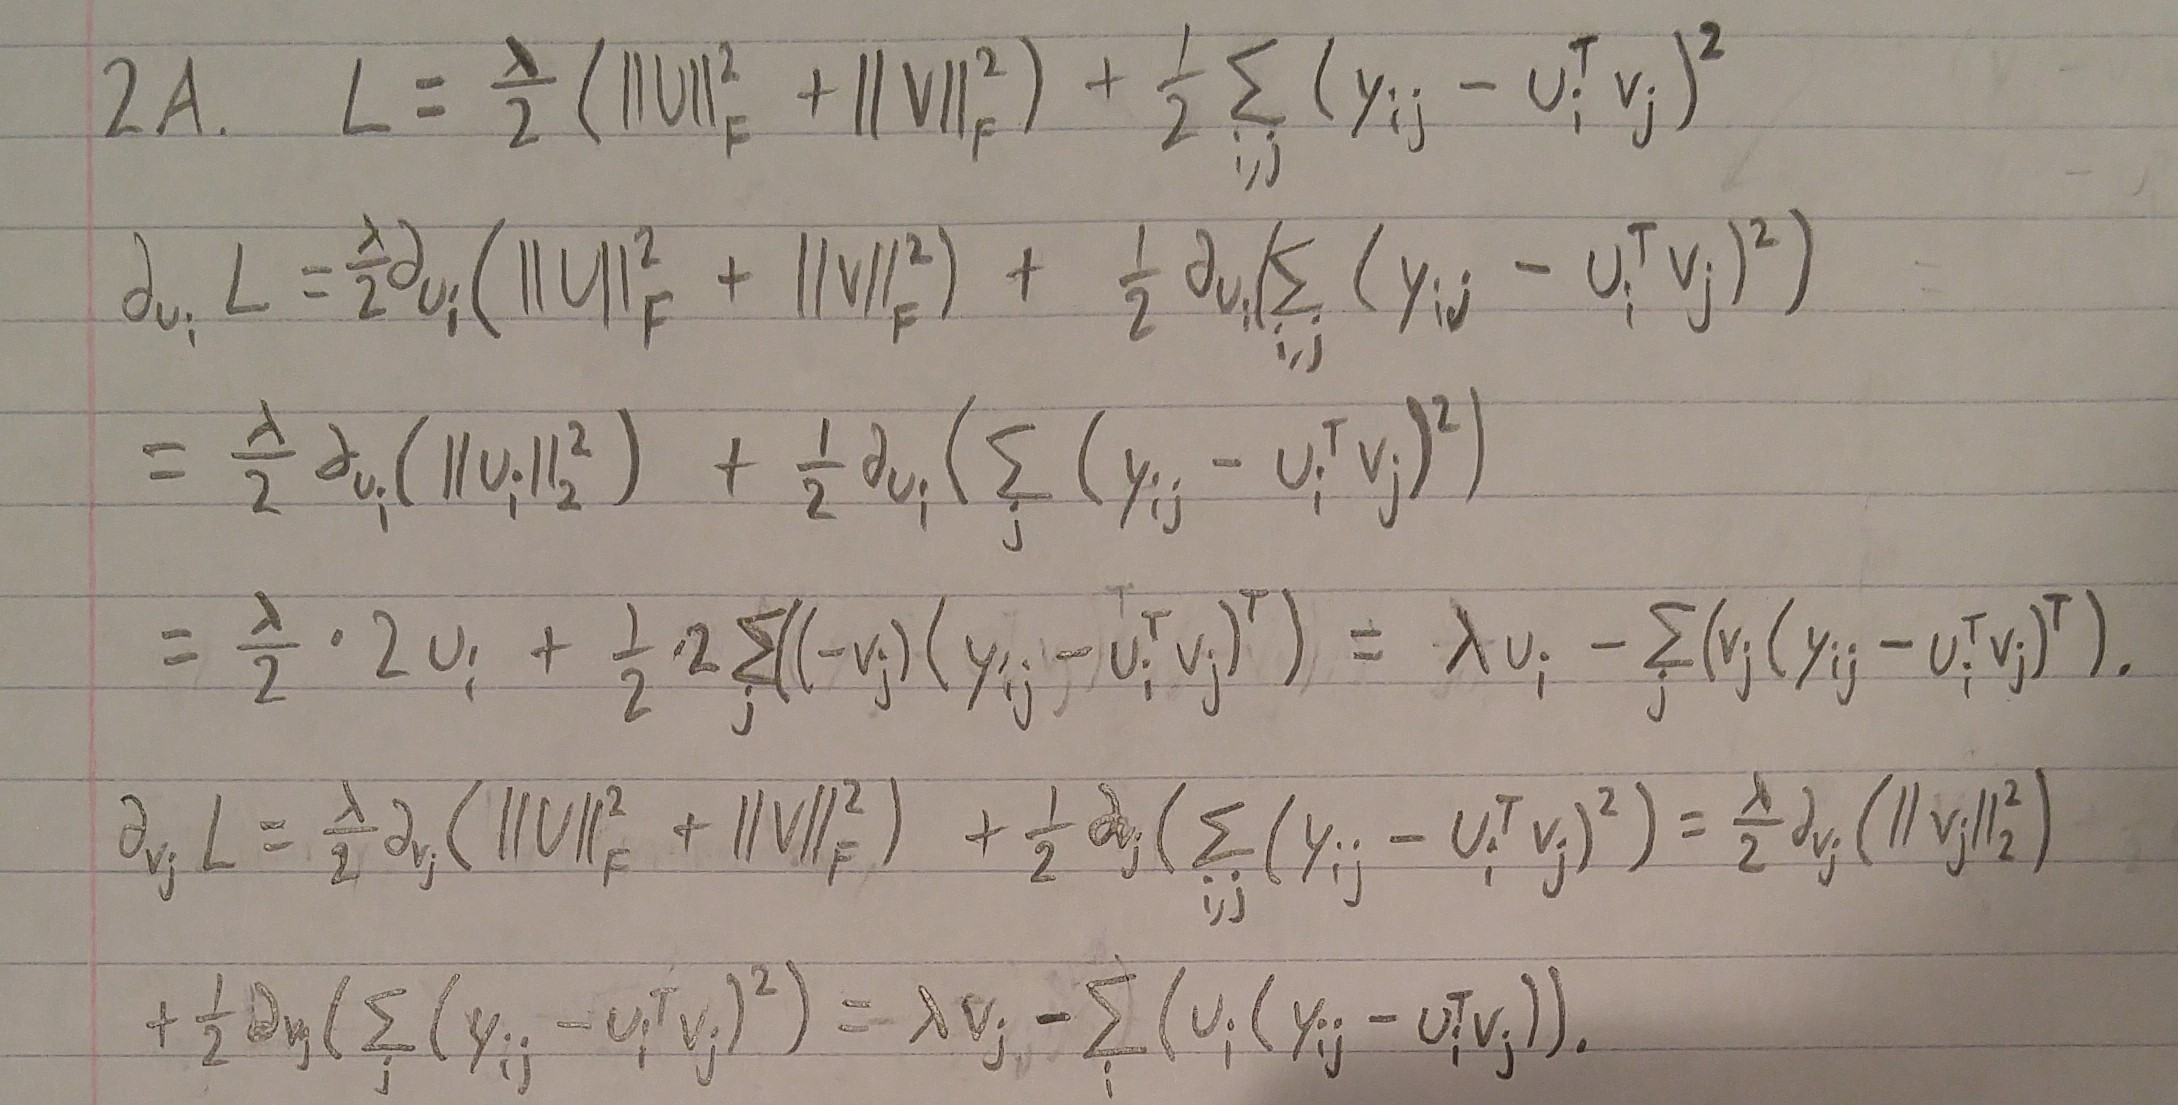
\includegraphics[scale=0.2]{../2a.jpg}
\end{figure}
\noindent
\end{solution}

\newpage
\problem[5]

\begin{solution}
\noindent
\begin{figure}[H]
\centering
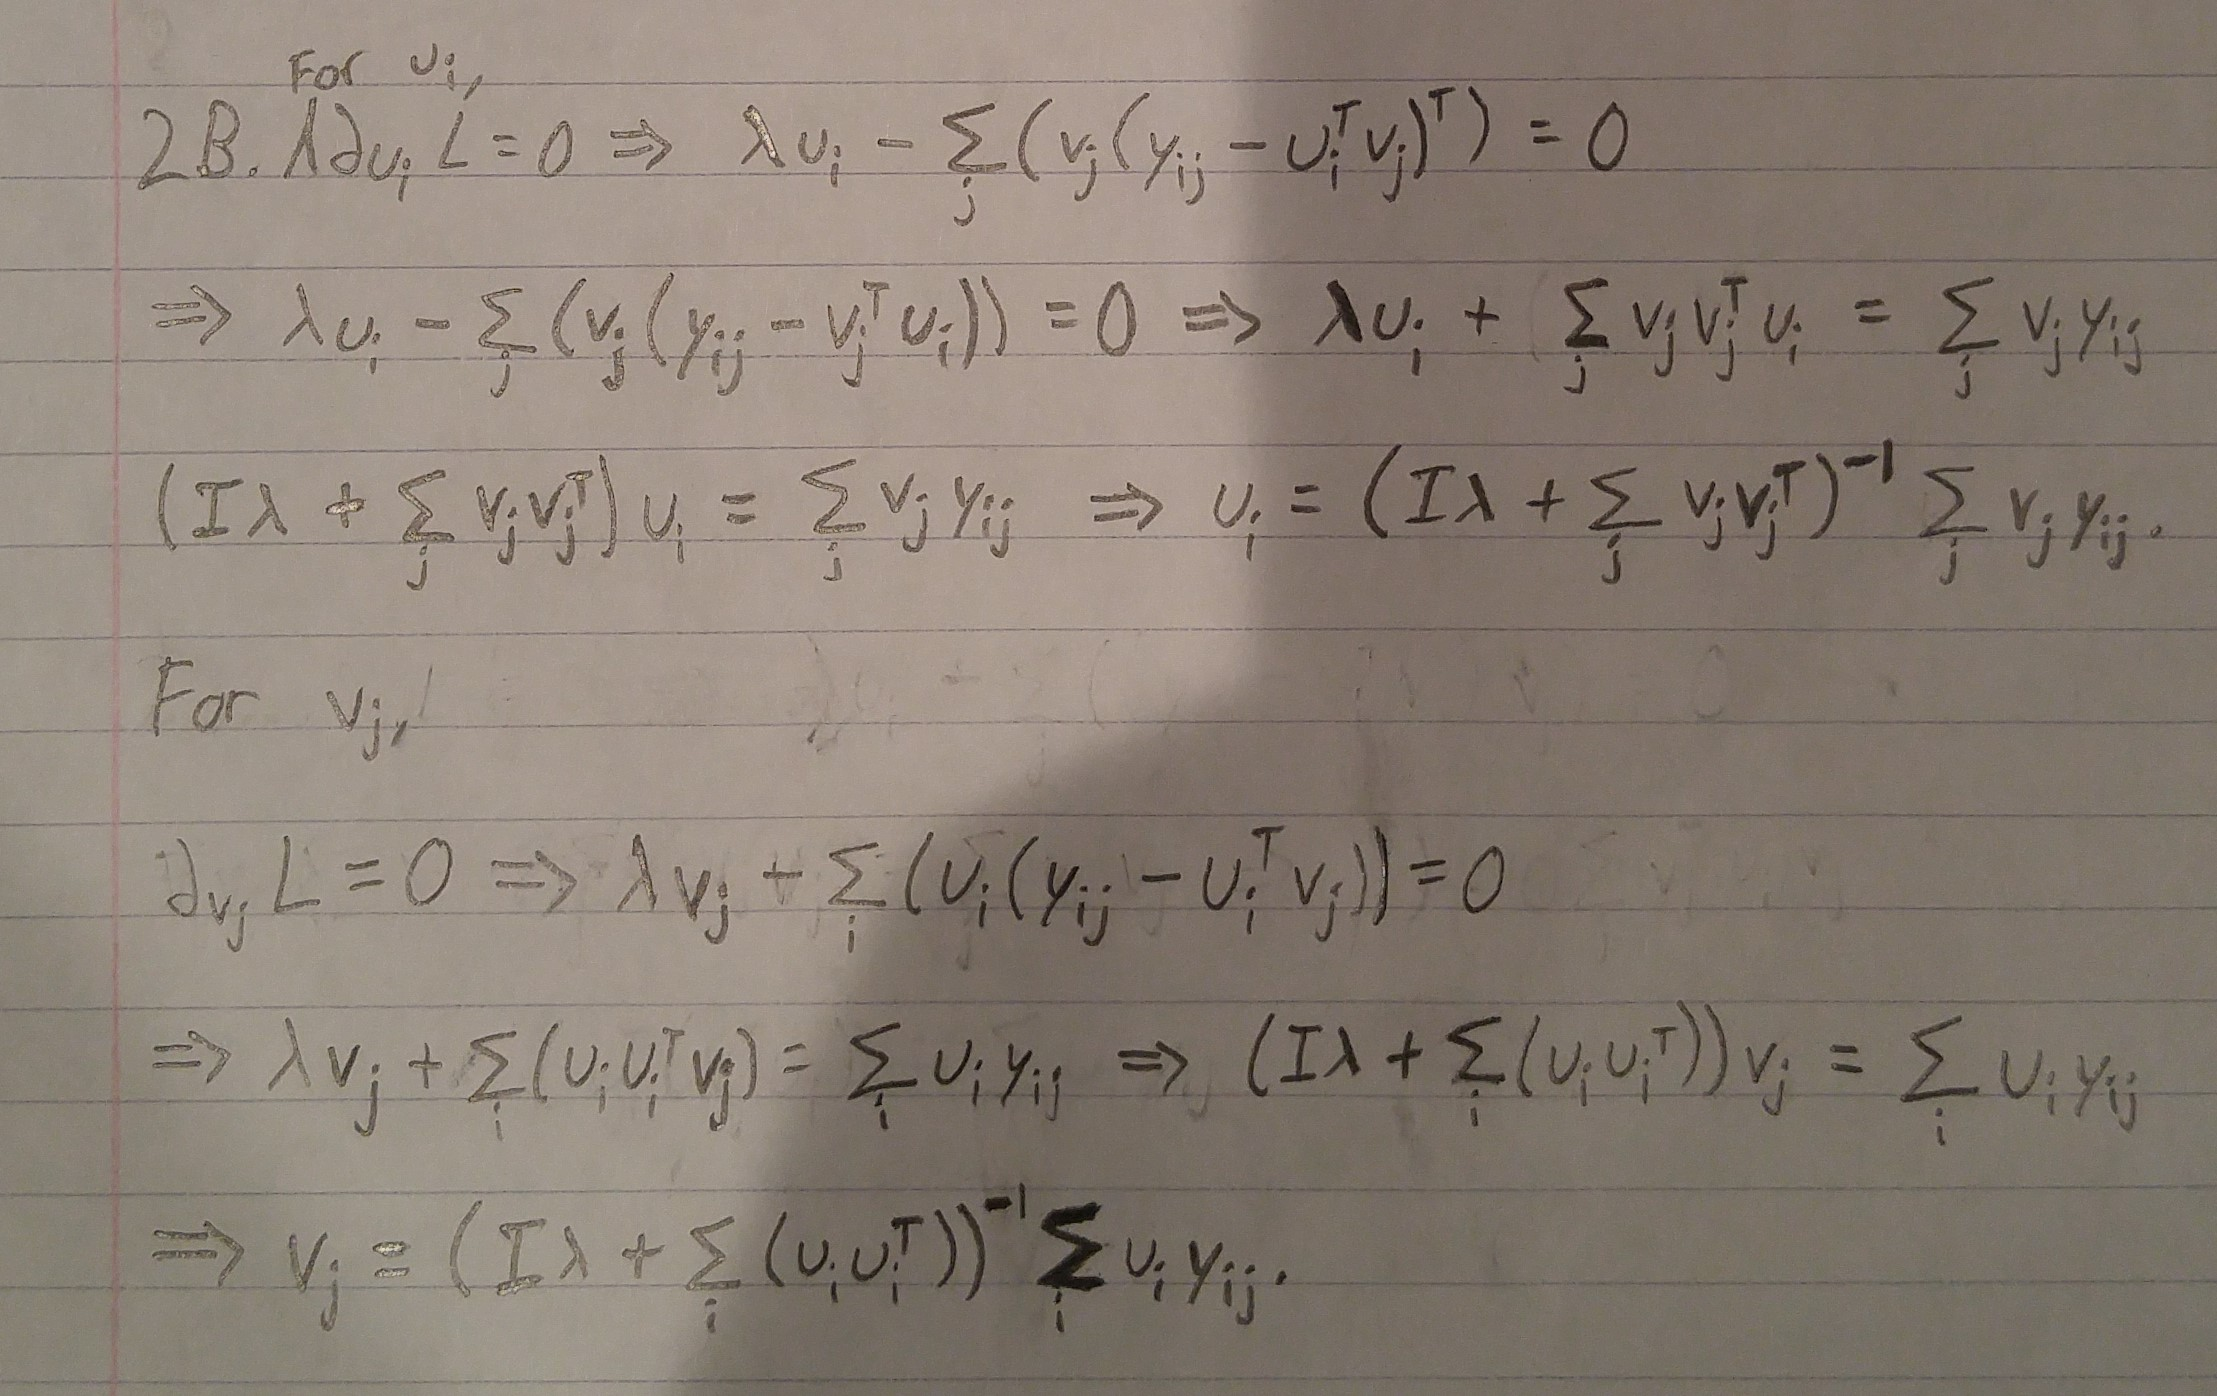
\includegraphics[scale=0.2]{../2b.jpg}
\end{figure}
\noindent
\end{solution}

\newpage
\problem[10]

\begin{solution}
See 2D.py and prob2utils.py for the solution code.
\end{solution}

\newpage
\problem[5]

\begin{solution}

%
%\begin{figure}[H]
%\begin{center}
%\includegraphics[width=0.8\textwidth]{plots/2d.png}
%\caption{Unregularized factorization}
%\label{fig:UnregFact}
%\end{center}
%\end{figure}


\end{solution}

\newpage
\problem[5]

\begin{solution}


%\begin{figure}[H]
%\begin{center}
%\includegraphics[width=0.45\textwidth]{plots/2e_ein.png}
%\caption{$E_{in}$ vs $k$ for different $\lambda$}
%\label{fig:RegFact1}
%\end{center}
%\end{figure}

%\begin{figure}[H]
%\begin{center}
%\includegraphics[width=0.45\textwidth]{plots/2e_eout.png}
%\caption{$E_{out}$ vs $k$ for different $\lambda$}
%\label{fig:RegFact2}
%\end{center}
%\end{figure}

 
\end{solution}






\newpage
\section{Word2Vec Principles [35 Points]}

\problem[5]


\begin{solution}\normalfont{
%Computing these gradients scales by a factor of $2s - 1$, since increasing $W$ by 1 adds $2s - 1$ gradients to compute, since for the extra word, $log p(w_{t+j} \vert w_t)$ has to be computed for all $-s \leq j \leq s, j \neq 0$.\\
%\\
Computing these gradients scales as $O(W^3)$, since gradients must be computed for every possible pair of $w$ vectors (this is $O(W^2)$), and since gradients must be computed for every word in the word list (this is $O(W)$).\\
\\
Since increasing $D$ increases the length of each $w$ vector, computing these gradients scales as $O(D)$, since if $d$ more dimensions are added to each $w$ vector, there are $d$ more pairs terms to multiply together with each gradient.\\
\\
In total, computing these gradients scales with $O(W^3D)$.
}\end{solution}


\newpage
\problem[10]

\begin{solution}
\noindent
\begin{figure}[H]
\centering
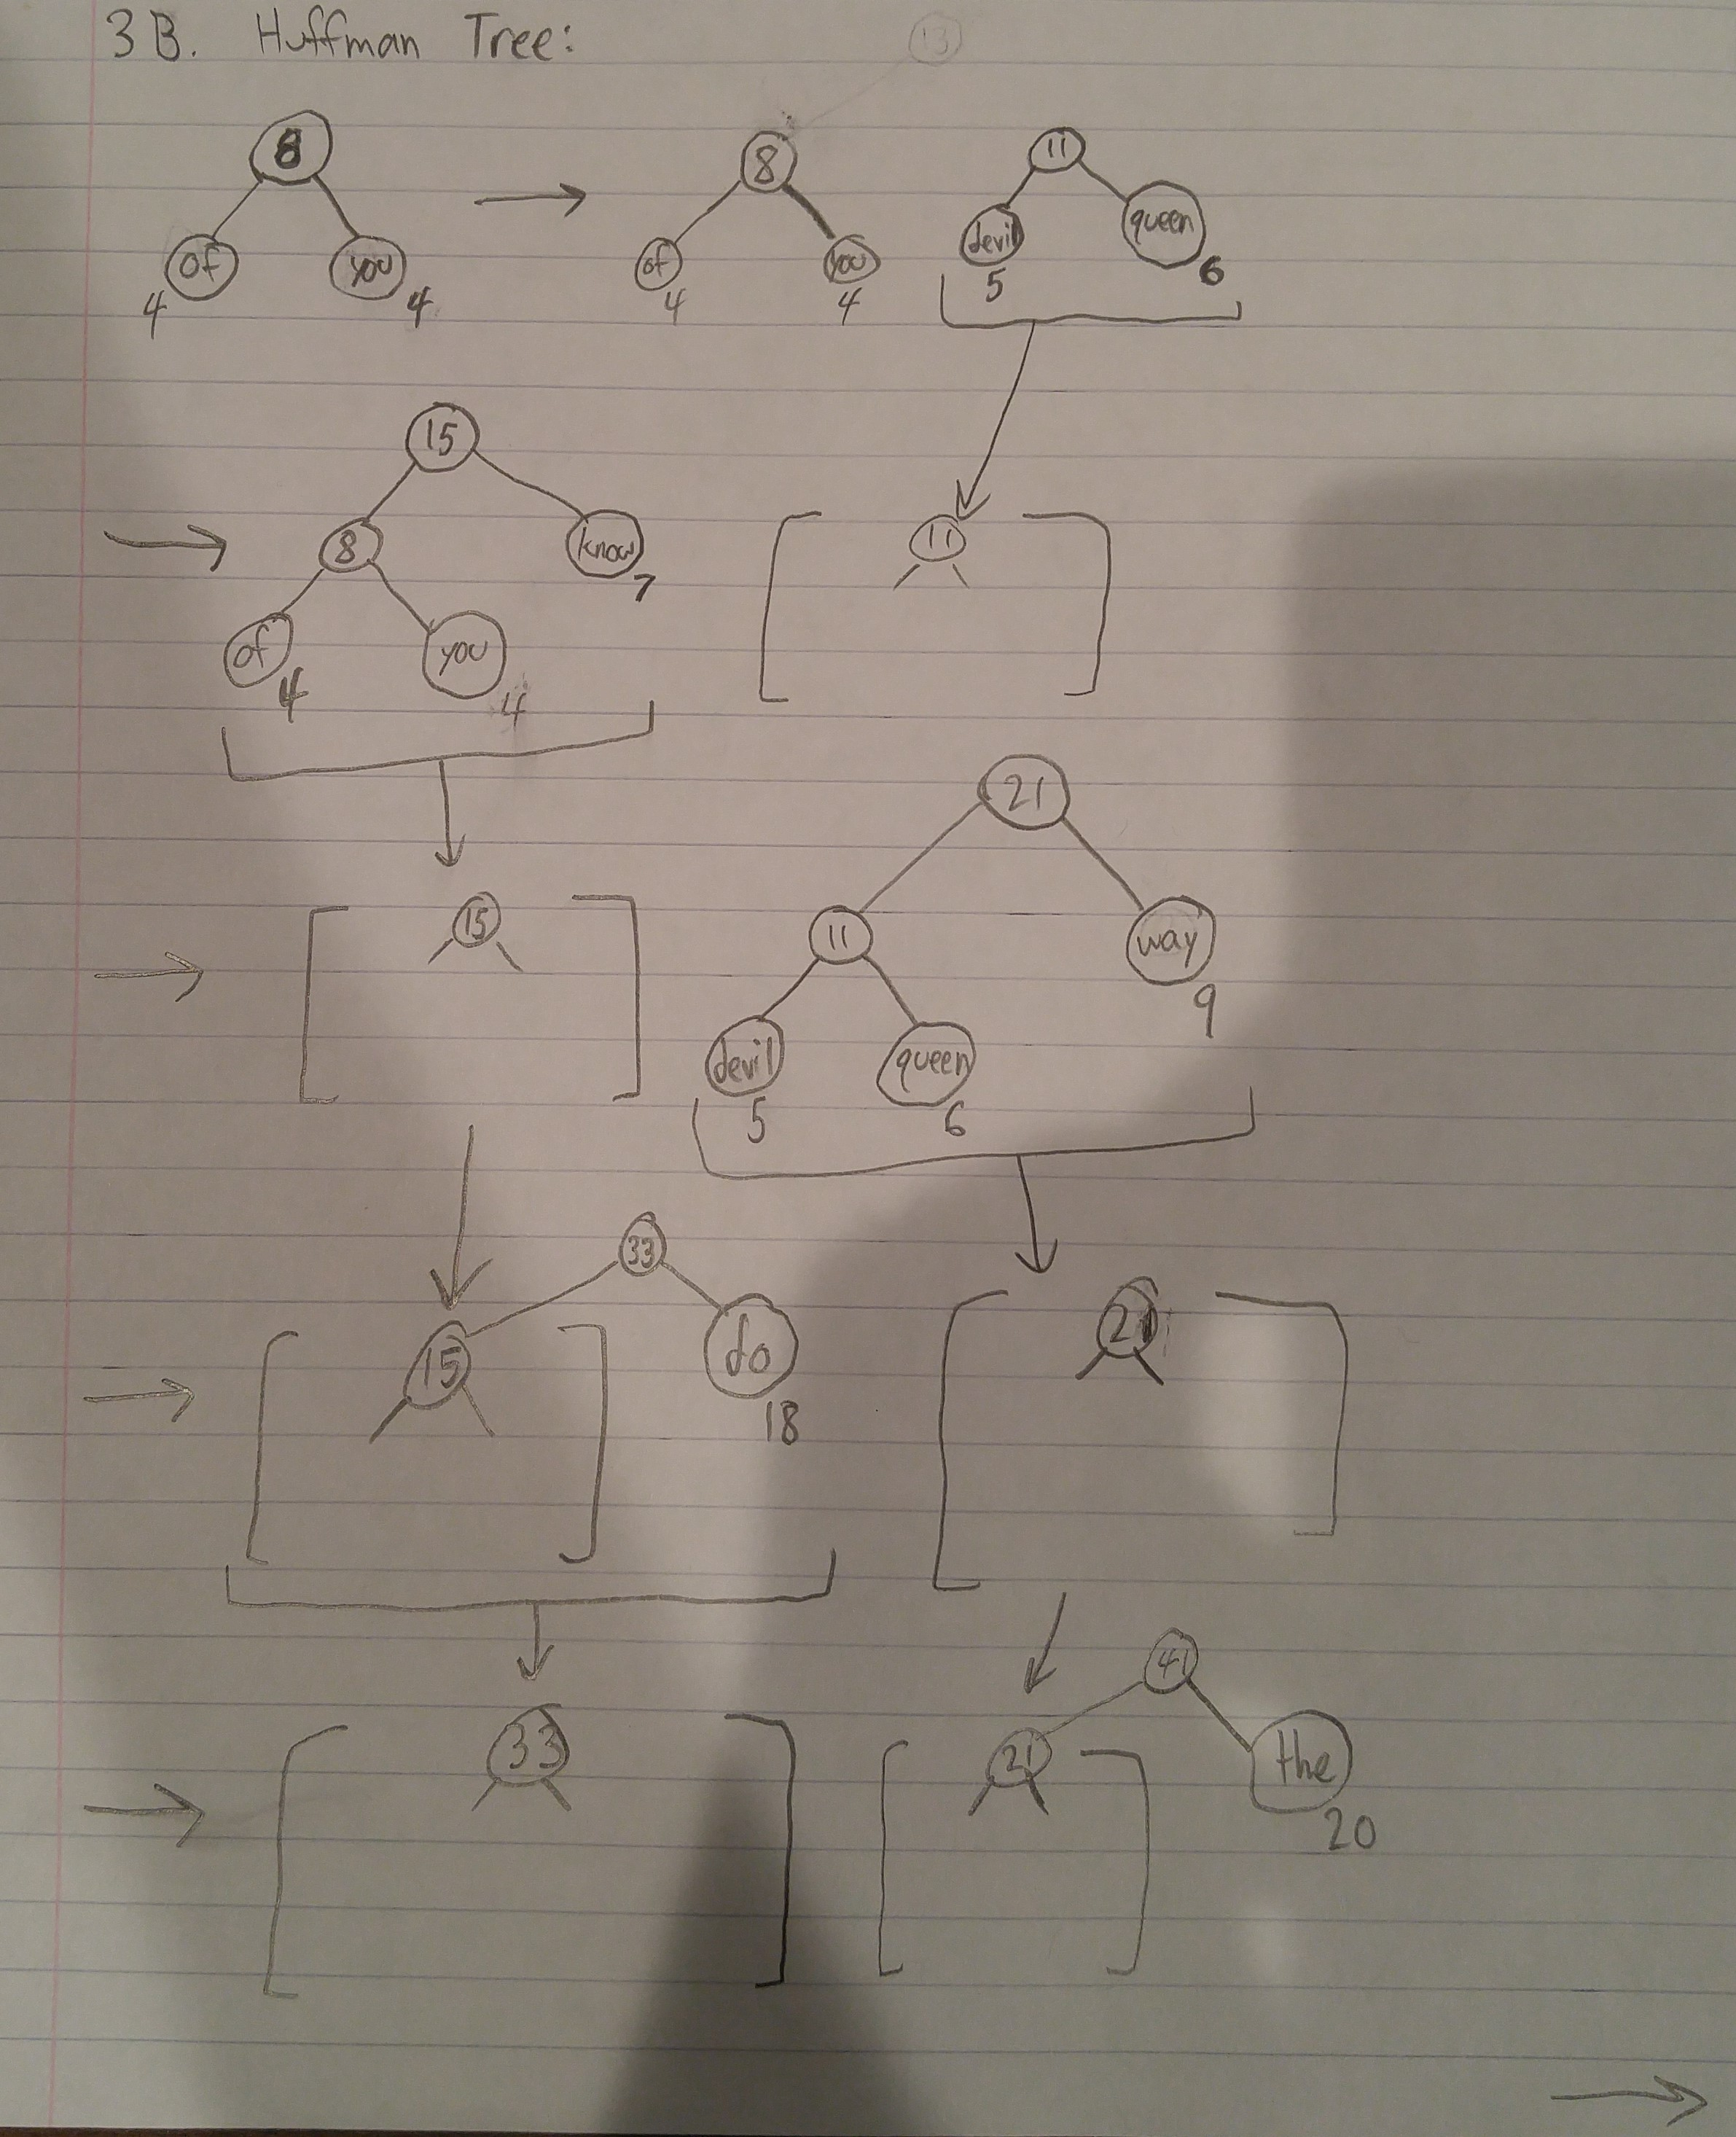
\includegraphics[scale=0.1]{../3b1.jpg}
\end{figure}
\noindent
\noindent
\begin{figure}[H]
\centering
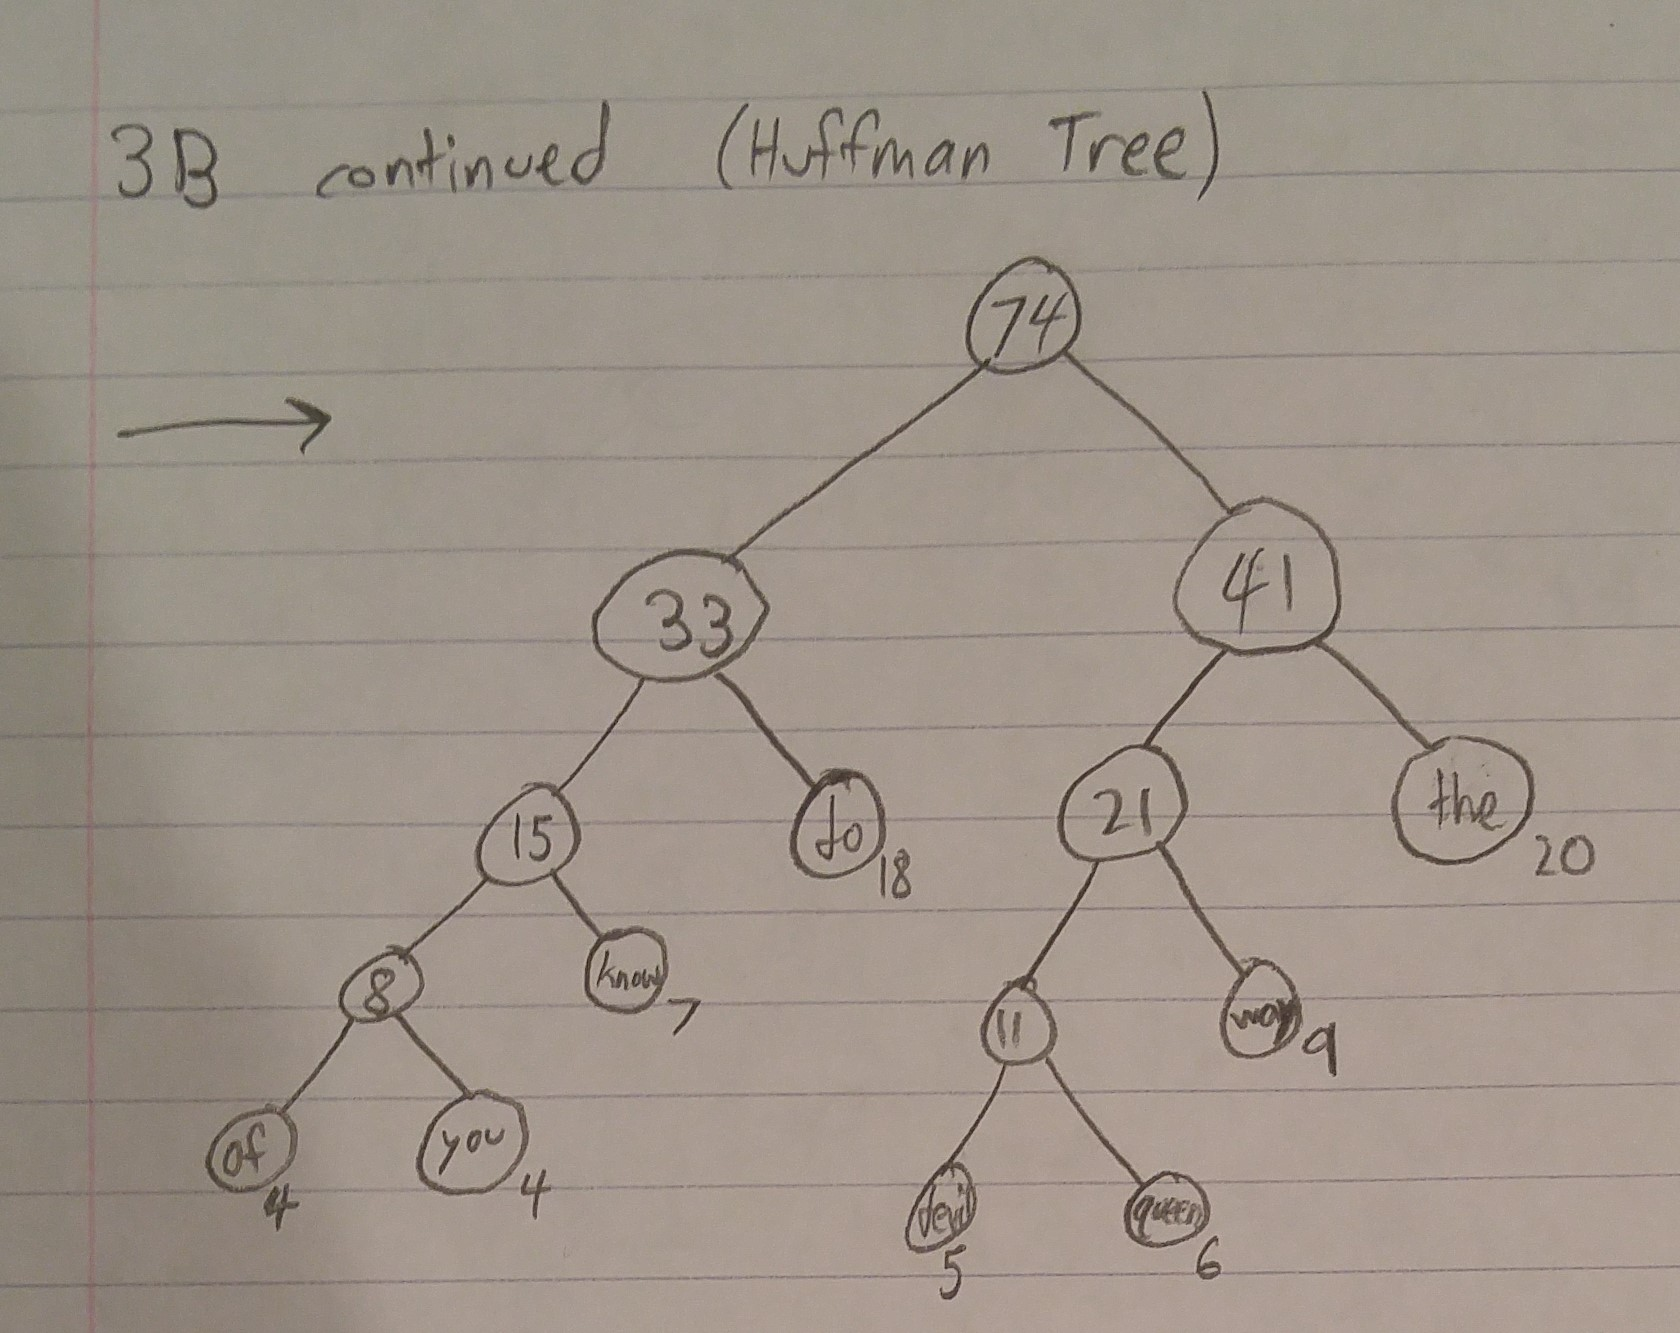
\includegraphics[scale=0.1]{../3b2.jpg}
\end{figure}
\noindent
\normalfont{The complete Huffman Tree is above.}
\end{solution}


\newpage
\problem[3]


\begin{solution}

\end{solution}




\newpage
\problem[10]



\begin{solution}
See solution code in P3C.py
\end{solution}


\newpage
\problem[2]


\begin{solution}

\end{solution}

\newpage
\problem[2]

\begin{solution}

\end{solution}

\newpage
\problem[1]

\begin{solution}

%\begin{verbatim}
%
%\end{verbatim}

\end{solution}
\newpage

\problem[2]

\begin{solution}


\end{solution}

\end{document}

